% Options for packages loaded elsewhere
\PassOptionsToPackage{unicode}{hyperref}
\PassOptionsToPackage{hyphens}{url}
%
\documentclass[
  11pt,
  ignorenonframetext,
]{beamer}
\usepackage{pgfpages}
\setbeamertemplate{caption}[numbered]
\setbeamertemplate{caption label separator}{: }
\setbeamercolor{caption name}{fg=normal text.fg}
\beamertemplatenavigationsymbolsempty
% Prevent slide breaks in the middle of a paragraph
\widowpenalties 1 10000
\raggedbottom
\setbeamertemplate{part page}{
  \centering
  \begin{beamercolorbox}[sep=16pt,center]{part title}
    \usebeamerfont{part title}\insertpart\par
  \end{beamercolorbox}
}
\setbeamertemplate{section page}{
  \centering
  \begin{beamercolorbox}[sep=12pt,center]{part title}
    \usebeamerfont{section title}\insertsection\par
  \end{beamercolorbox}
}
\setbeamertemplate{subsection page}{
  \centering
  \begin{beamercolorbox}[sep=8pt,center]{part title}
    \usebeamerfont{subsection title}\insertsubsection\par
  \end{beamercolorbox}
}
\AtBeginPart{
  \frame{\partpage}
}
\AtBeginSection{
  \ifbibliography
  \else
    \frame{\sectionpage}
  \fi
}
\AtBeginSubsection{
  \frame{\subsectionpage}
}
\usepackage{amsmath,amssymb}
\usepackage{lmodern}
\usepackage{iftex}
\ifPDFTeX
  \usepackage[T1]{fontenc}
  \usepackage[utf8]{inputenc}
  \usepackage{textcomp} % provide euro and other symbols
\else % if luatex or xetex
  \usepackage{unicode-math}
  \defaultfontfeatures{Scale=MatchLowercase}
  \defaultfontfeatures[\rmfamily]{Ligatures=TeX,Scale=1}
\fi
\usetheme[]{metropolis}
% Use upquote if available, for straight quotes in verbatim environments
\IfFileExists{upquote.sty}{\usepackage{upquote}}{}
\IfFileExists{microtype.sty}{% use microtype if available
  \usepackage[]{microtype}
  \UseMicrotypeSet[protrusion]{basicmath} % disable protrusion for tt fonts
}{}
\makeatletter
\@ifundefined{KOMAClassName}{% if non-KOMA class
  \IfFileExists{parskip.sty}{%
    \usepackage{parskip}
  }{% else
    \setlength{\parindent}{0pt}
    \setlength{\parskip}{6pt plus 2pt minus 1pt}}
}{% if KOMA class
  \KOMAoptions{parskip=half}}
\makeatother
\usepackage{xcolor}
\newif\ifbibliography
\usepackage{color}
\usepackage{fancyvrb}
\newcommand{\VerbBar}{|}
\newcommand{\VERB}{\Verb[commandchars=\\\{\}]}
\DefineVerbatimEnvironment{Highlighting}{Verbatim}{commandchars=\\\{\}}
% Add ',fontsize=\small' for more characters per line
\newenvironment{Shaded}{}{}
\newcommand{\AlertTok}[1]{\textcolor[rgb]{1.00,0.00,0.00}{\textbf{#1}}}
\newcommand{\AnnotationTok}[1]{\textcolor[rgb]{0.38,0.63,0.69}{\textbf{\textit{#1}}}}
\newcommand{\AttributeTok}[1]{\textcolor[rgb]{0.49,0.56,0.16}{#1}}
\newcommand{\BaseNTok}[1]{\textcolor[rgb]{0.25,0.63,0.44}{#1}}
\newcommand{\BuiltInTok}[1]{#1}
\newcommand{\CharTok}[1]{\textcolor[rgb]{0.25,0.44,0.63}{#1}}
\newcommand{\CommentTok}[1]{\textcolor[rgb]{0.38,0.63,0.69}{\textit{#1}}}
\newcommand{\CommentVarTok}[1]{\textcolor[rgb]{0.38,0.63,0.69}{\textbf{\textit{#1}}}}
\newcommand{\ConstantTok}[1]{\textcolor[rgb]{0.53,0.00,0.00}{#1}}
\newcommand{\ControlFlowTok}[1]{\textcolor[rgb]{0.00,0.44,0.13}{\textbf{#1}}}
\newcommand{\DataTypeTok}[1]{\textcolor[rgb]{0.56,0.13,0.00}{#1}}
\newcommand{\DecValTok}[1]{\textcolor[rgb]{0.25,0.63,0.44}{#1}}
\newcommand{\DocumentationTok}[1]{\textcolor[rgb]{0.73,0.13,0.13}{\textit{#1}}}
\newcommand{\ErrorTok}[1]{\textcolor[rgb]{1.00,0.00,0.00}{\textbf{#1}}}
\newcommand{\ExtensionTok}[1]{#1}
\newcommand{\FloatTok}[1]{\textcolor[rgb]{0.25,0.63,0.44}{#1}}
\newcommand{\FunctionTok}[1]{\textcolor[rgb]{0.02,0.16,0.49}{#1}}
\newcommand{\ImportTok}[1]{#1}
\newcommand{\InformationTok}[1]{\textcolor[rgb]{0.38,0.63,0.69}{\textbf{\textit{#1}}}}
\newcommand{\KeywordTok}[1]{\textcolor[rgb]{0.00,0.44,0.13}{\textbf{#1}}}
\newcommand{\NormalTok}[1]{#1}
\newcommand{\OperatorTok}[1]{\textcolor[rgb]{0.40,0.40,0.40}{#1}}
\newcommand{\OtherTok}[1]{\textcolor[rgb]{0.00,0.44,0.13}{#1}}
\newcommand{\PreprocessorTok}[1]{\textcolor[rgb]{0.74,0.48,0.00}{#1}}
\newcommand{\RegionMarkerTok}[1]{#1}
\newcommand{\SpecialCharTok}[1]{\textcolor[rgb]{0.25,0.44,0.63}{#1}}
\newcommand{\SpecialStringTok}[1]{\textcolor[rgb]{0.73,0.40,0.53}{#1}}
\newcommand{\StringTok}[1]{\textcolor[rgb]{0.25,0.44,0.63}{#1}}
\newcommand{\VariableTok}[1]{\textcolor[rgb]{0.10,0.09,0.49}{#1}}
\newcommand{\VerbatimStringTok}[1]{\textcolor[rgb]{0.25,0.44,0.63}{#1}}
\newcommand{\WarningTok}[1]{\textcolor[rgb]{0.38,0.63,0.69}{\textbf{\textit{#1}}}}
\usepackage{graphicx}
\makeatletter
\def\maxwidth{\ifdim\Gin@nat@width>\linewidth\linewidth\else\Gin@nat@width\fi}
\def\maxheight{\ifdim\Gin@nat@height>\textheight\textheight\else\Gin@nat@height\fi}
\makeatother
% Scale images if necessary, so that they will not overflow the page
% margins by default, and it is still possible to overwrite the defaults
% using explicit options in \includegraphics[width, height, ...]{}
\setkeys{Gin}{width=\maxwidth,height=\maxheight,keepaspectratio}
% Set default figure placement to htbp
\makeatletter
\def\fps@figure{htbp}
\makeatother
\setlength{\emergencystretch}{3em} % prevent overfull lines
\providecommand{\tightlist}{%
  \setlength{\itemsep}{0pt}\setlength{\parskip}{0pt}}
\setcounter{secnumdepth}{-\maxdimen} % remove section numbering
\ifLuaTeX
  \usepackage{selnolig}  % disable illegal ligatures
\fi
\IfFileExists{bookmark.sty}{\usepackage{bookmark}}{\usepackage{hyperref}}
\IfFileExists{xurl.sty}{\usepackage{xurl}}{} % add URL line breaks if available
\urlstyle{same} % disable monospaced font for URLs
\hypersetup{
  pdftitle={Análisis de presencias con procesos de puntos},
  pdfauthor={Gerardo Martín},
  hidelinks,
  pdfcreator={LaTeX via pandoc}}

\title{Análisis de presencias con procesos de puntos}
\subtitle{Tutorial básico de spatstat}
\author{Gerardo Martín}
\date{2022-06-29}

\begin{document}
\frame{\titlepage}

\hypertarget{introducciuxf3n}{%
\section{Introducción}\label{introducciuxf3n}}

\begin{frame}[fragile]{¿Qué es \texttt{spatstat}?}
\protect\hypertarget{quuxe9-es-spatstat}{}
\begin{itemize}
\item
  \texttt{spat} = Spatial
\item
  \texttt{stat} = Statistics
\item
  Paquete de \textbf{R} para hacer estadística espacial de procesos de
  puntos

  \begin{itemize}
  \tightlist
  \item
    Sintaxis típica de R básico
  \item
    Objetos específicos del paquete
  \end{itemize}
\end{itemize}
\end{frame}

\begin{frame}{Libro}
\protect\hypertarget{libro}{}
Por desarrolladores del paquete

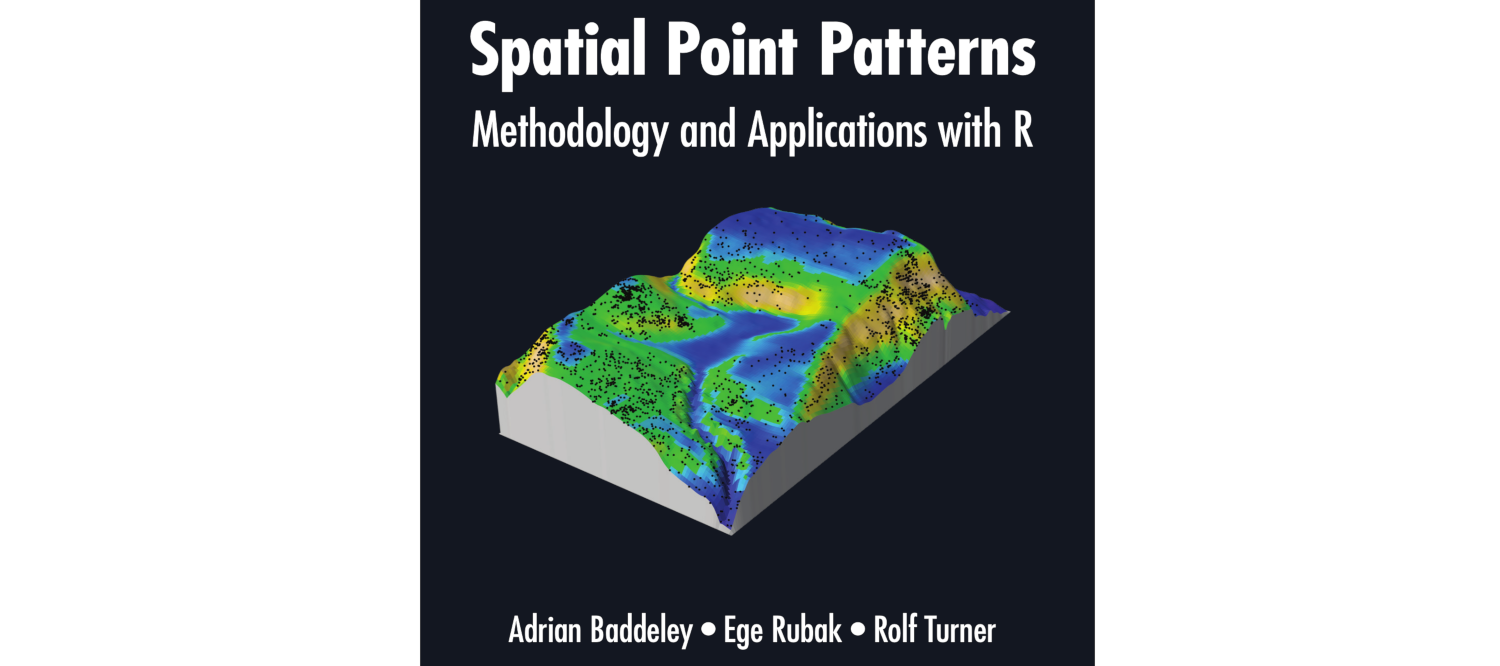
\includegraphics{Figuras/Spat-book.png}
\end{frame}

\begin{frame}[fragile]{¿Qué veremos aquí?}
\protect\hypertarget{quuxe9-veremos-aquuxed}{}
\begin{enumerate}
\item
  Instalación y carga
\item
  Formateo
\item
  Transformación de otros paquetes a \texttt{spatstat}
\item
  Análisis exploratorio

  4.1. Detección de autocorrelación 4.2. Análisis de respuesta a
  covariables 4.3. Propuesta de modelos en relación a covariables
\item
  Ajuste de modelo
\end{enumerate}
\end{frame}

\hypertarget{instalaciuxf3n-y-carga}{%
\section{Instalación y carga}\label{instalaciuxf3n-y-carga}}

\begin{frame}[fragile]{Igual que cualquier paquete de \textbf{R}}
\protect\hypertarget{igual-que-cualquier-paquete-de-r}{}
Instalación

\begin{Shaded}
\begin{Highlighting}[]
\FunctionTok{install.packages}\NormalTok{(}\StringTok{"spatstat"}\NormalTok{)}
\end{Highlighting}
\end{Shaded}

Carga

\begin{Shaded}
\begin{Highlighting}[]
\FunctionTok{library}\NormalTok{(spatstat)}
\end{Highlighting}
\end{Shaded}
\end{frame}

\begin{frame}[fragile]{Peeero}
\protect\hypertarget{peeero}{}
Necesitamos también (para leer raster de covariables):

\begin{Shaded}
\begin{Highlighting}[]
\FunctionTok{library}\NormalTok{(rgdal)}
\FunctionTok{library}\NormalTok{(raster)}
\FunctionTok{library}\NormalTok{(foreach)}
\end{Highlighting}
\end{Shaded}
\end{frame}

\hypertarget{formateo}{%
\section{Formateo}\label{formateo}}

\begin{frame}{Liga para los datos}
\protect\hypertarget{liga-para-los-datos}{}
\href{Datos-ejemplos/Covariables.zip}{Variables ambientales}
\end{frame}

\begin{frame}[fragile]{Carga de rasters}
\protect\hypertarget{carga-de-rasters}{}
\begin{Shaded}
\begin{Highlighting}[]
\NormalTok{archivos }\OtherTok{\textless{}{-}} \FunctionTok{list.files}\NormalTok{(}\StringTok{"Datos{-}ejemplos/"}\NormalTok{, }\StringTok{"tif"}\NormalTok{, }
                       \AttributeTok{full.names =}\NormalTok{ T, }
                       \AttributeTok{recursive =}\NormalTok{ F)}
\NormalTok{r }\OtherTok{\textless{}{-}} \FunctionTok{stack}\NormalTok{(archivos)}
\end{Highlighting}
\end{Shaded}

\begin{Shaded}
\begin{Highlighting}[]
\FunctionTok{plot}\NormalTok{(r[[}\DecValTok{1}\NormalTok{]])}
\end{Highlighting}
\end{Shaded}

\begin{center}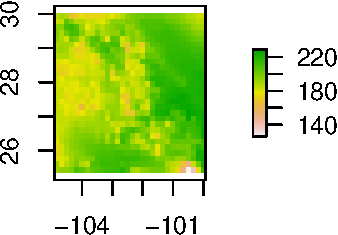
\includegraphics{Tutorial-spatstat_files/figure-beamer/unnamed-chunk-6-1} \end{center}
\end{frame}

\begin{frame}[fragile]{Transformar de \texttt{raster} a \texttt{im}}
\protect\hypertarget{transformar-de-raster-a-im}{}
Si hacemos:

\begin{Shaded}
\begin{Highlighting}[]
\FunctionTok{class}\NormalTok{(r)}
\end{Highlighting}
\end{Shaded}

\begin{verbatim}
## [1] "RasterStack"
## attr(,"package")
## [1] "raster"
\end{verbatim}

vemos que el tipo de objeto es \texttt{raster}, pero \texttt{spastat}
utiliza \texttt{im}

Transformación en lote con
\href{Funciones-spatstat/imFromStack.R}{\texttt{imFromStack}}
\end{frame}

\begin{frame}[fragile]{Transformar de \texttt{raster} a \texttt{im}}
\protect\hypertarget{transformar-de-raster-a-im-1}{}
Para cargar \texttt{imFromStack}:

\begin{Shaded}
\begin{Highlighting}[]
\FunctionTok{source}\NormalTok{(}\StringTok{"Funciones{-}spatstat/imFromStack.R"}\NormalTok{)}
\end{Highlighting}
\end{Shaded}

Y se usa:

\begin{Shaded}
\begin{Highlighting}[]
\NormalTok{r.im }\OtherTok{\textless{}{-}} \FunctionTok{imFromStack}\NormalTok{(r)}
\FunctionTok{class}\NormalTok{(r.im)}
\end{Highlighting}
\end{Shaded}

\begin{verbatim}
## [1] "list"
\end{verbatim}
\end{frame}

\begin{frame}[fragile]{Ventana de trabajo}
\protect\hypertarget{ventana-de-trabajo}{}
Cálculo de intensidad se hace con la ``ventana''. Utilizaremos la
función
\href{Funciones-spatstat/winFromRaster.R}{\texttt{winFromRaster}}:

\begin{Shaded}
\begin{Highlighting}[]
\FunctionTok{source}\NormalTok{(}\StringTok{"Funciones{-}spatstat/winFromRaster.R"}\NormalTok{)}
\NormalTok{w }\OtherTok{\textless{}{-}} \FunctionTok{winFromRaster}\NormalTok{(r)}
\end{Highlighting}
\end{Shaded}

Para verificar la clase del objeto:

\begin{Shaded}
\begin{Highlighting}[]
\FunctionTok{class}\NormalTok{(w)}
\end{Highlighting}
\end{Shaded}

\begin{verbatim}
## [1] "owin"
\end{verbatim}
\end{frame}

\begin{frame}[fragile]{Puntos de ocurrencia}
\protect\hypertarget{puntos-de-ocurrencia}{}
Vamos a simular las coordenadas \(x\) y \(y\) de un proceso de puntos:

\begin{Shaded}
\begin{Highlighting}[]
\FunctionTok{set.seed}\NormalTok{(}\DecValTok{984573}\NormalTok{)}
\NormalTok{puntos }\OtherTok{\textless{}{-}} \FunctionTok{data.frame}\NormalTok{(}\FunctionTok{coordinates}\NormalTok{(r)[}\FunctionTok{sample}\NormalTok{(}\DecValTok{1}\SpecialCharTok{:}\DecValTok{840}\NormalTok{, }\DecValTok{200}\NormalTok{),])}
\NormalTok{puntos}\SpecialCharTok{$}\NormalTok{x }\OtherTok{\textless{}{-}}\NormalTok{ puntos}\SpecialCharTok{$}\NormalTok{x }\SpecialCharTok{+} \FunctionTok{rnorm}\NormalTok{(}\DecValTok{200}\NormalTok{, }\DecValTok{0}\NormalTok{, }\FloatTok{0.05}\NormalTok{)}
\NormalTok{puntos}\SpecialCharTok{$}\NormalTok{y }\OtherTok{\textless{}{-}}\NormalTok{ puntos}\SpecialCharTok{$}\NormalTok{y }\SpecialCharTok{+} \FunctionTok{rnorm}\NormalTok{(}\DecValTok{200}\NormalTok{, }\DecValTok{0}\NormalTok{, }\FloatTok{0.05}\NormalTok{)}
\end{Highlighting}
\end{Shaded}

El formato que requiere \texttt{spatstat} es \texttt{ppp}:

\begin{Shaded}
\begin{Highlighting}[]
\NormalTok{puntos.ppp }\OtherTok{\textless{}{-}} \FunctionTok{ppp}\NormalTok{(}\AttributeTok{x =}\NormalTok{ puntos}\SpecialCharTok{$}\NormalTok{x,}
                  \AttributeTok{y =}\NormalTok{ puntos}\SpecialCharTok{$}\NormalTok{y,}
                  \AttributeTok{window =}\NormalTok{ w,}
                  \AttributeTok{check =}\NormalTok{ F)}
\FunctionTok{class}\NormalTok{(puntos.ppp)}
\end{Highlighting}
\end{Shaded}

\begin{verbatim}
## [1] "ppp"
\end{verbatim}
\end{frame}

\begin{frame}[fragile]{Puntos de ocurrencia}
\protect\hypertarget{puntos-de-ocurrencia-1}{}
\begin{Shaded}
\begin{Highlighting}[]
\FunctionTok{plot}\NormalTok{(puntos.ppp)}
\end{Highlighting}
\end{Shaded}

\begin{center}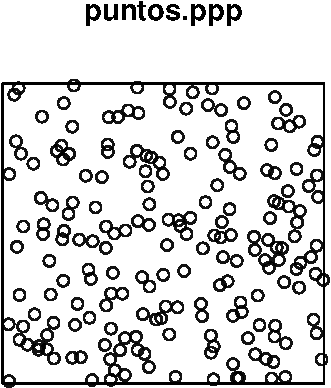
\includegraphics{Tutorial-spatstat_files/figure-beamer/unnamed-chunk-14-1} \end{center}
\end{frame}

\hypertarget{anuxe1lisis-exploratorio}{%
\section{Análisis exploratorio}\label{anuxe1lisis-exploratorio}}

\begin{frame}{Detección/medición de autocorrelación}
\protect\hypertarget{detecciuxf3nmediciuxf3n-de-autocorrelaciuxf3n}{}
\begin{itemize}
\tightlist
\item
  Análisis visual
\end{itemize}

\begin{center}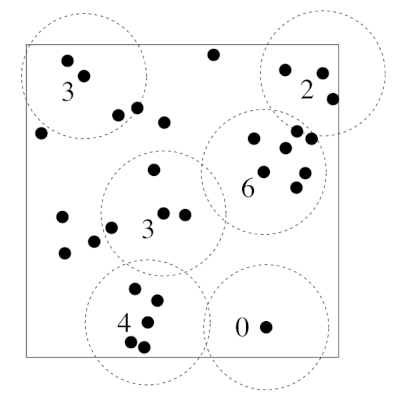
\includegraphics{Figuras/Cuenta-vecinos} \end{center}
\end{frame}

\begin{frame}{Función de Ripley}
\protect\hypertarget{funciuxf3n-de-ripley}{}
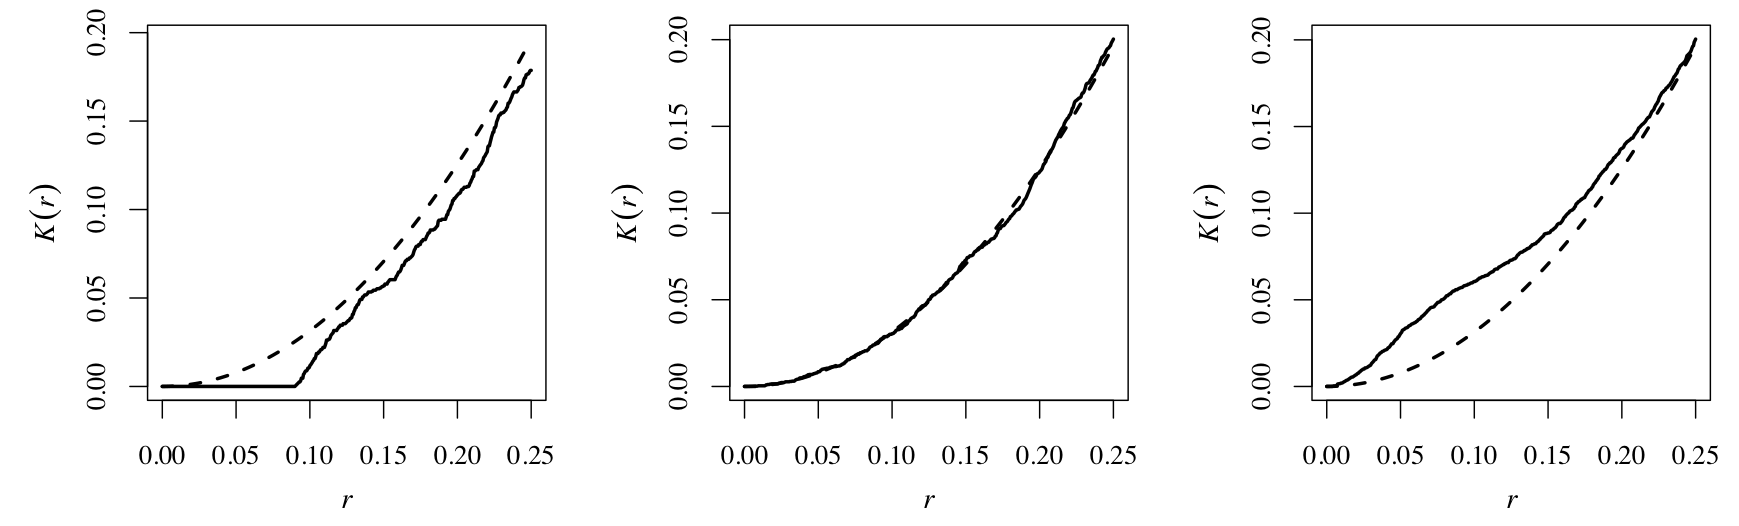
\includegraphics{Figuras/K-Ripley.png}
\end{frame}

\begin{frame}[fragile]{Función de Ripley}
\protect\hypertarget{funciuxf3n-de-ripley-1}{}
\begin{Shaded}
\begin{Highlighting}[]
\NormalTok{K }\OtherTok{\textless{}{-}} \FunctionTok{envelope}\NormalTok{(puntos.ppp, }\AttributeTok{fun =}\NormalTok{ Kest, }\AttributeTok{nsim =} \DecValTok{39}\NormalTok{)}
\end{Highlighting}
\end{Shaded}

\begin{itemize}
\tightlist
\item
  \texttt{puntos.ppp} objeto que contiene los puntos
\item
  \texttt{fun\ =\ Kest} función que se estimará
\item
  \texttt{nsim\ =\ 39} número de simulaciones para IC al 95\%
\end{itemize}
\end{frame}

\begin{frame}[fragile]{Función de Ripley}
\protect\hypertarget{funciuxf3n-de-ripley-2}{}
\begin{Shaded}
\begin{Highlighting}[]
\NormalTok{K }\OtherTok{\textless{}{-}} \FunctionTok{envelope}\NormalTok{(puntos.ppp, }\AttributeTok{fun =}\NormalTok{ Kest, }\AttributeTok{nsim =} \DecValTok{39}\NormalTok{)}
\FunctionTok{plot}\NormalTok{(K)}
\end{Highlighting}
\end{Shaded}

\begin{center}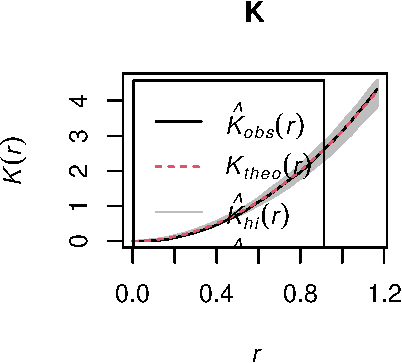
\includegraphics{Tutorial-spatstat_files/figure-beamer/unnamed-chunk-18-1} \end{center}
\end{frame}

\begin{frame}[fragile]{Análisis de respuesta a covariables}
\protect\hypertarget{anuxe1lisis-de-respuesta-a-covariables}{}
\begin{itemize}
\item
  Función \texttt{rhohat} de \texttt{spatstat}

  \begin{itemize}
  \tightlist
  \item
    Gráfica de intensidad en relación a covariable
  \item
    Suavizada
  \end{itemize}
\item
  Implementada en lotes con
  \href{Funciones-spatstat/plotQuantIntens.R}{plotQuantIntens}
\end{itemize}
\end{frame}

\begin{frame}[fragile]{Análisis de respuesta a covariables}
\protect\hypertarget{anuxe1lisis-de-respuesta-a-covariables-1}{}
Uso de \texttt{plotQuantIntens}:

\begin{Shaded}
\begin{Highlighting}[]
\NormalTok{Q }\OtherTok{\textless{}{-}} \FunctionTok{pixelquad}\NormalTok{(}\AttributeTok{X =}\NormalTok{ puntos.ppp, }\AttributeTok{W =} \FunctionTok{as.owin}\NormalTok{(w))}

\FunctionTok{source}\NormalTok{(}\StringTok{"Funciones{-}spatstat/plotQuantIntens.R"}\NormalTok{)}
\FunctionTok{plotQuantIntens}\NormalTok{(}\AttributeTok{imList =}\NormalTok{ r.im,}
                \AttributeTok{noCuts =} \DecValTok{5}\NormalTok{,}
                \AttributeTok{Quad =}\NormalTok{ Q,}
                \AttributeTok{p.pp =}\NormalTok{ puntos.ppp,}
                \AttributeTok{dir =} \StringTok{""}\NormalTok{,}
                \AttributeTok{name =} \StringTok{"Respuestas"}\NormalTok{)}
\end{Highlighting}
\end{Shaded}

\begin{verbatim}
## pdf 
##   2
\end{verbatim}
\end{frame}

\hypertarget{ajuste-del-modelo}{%
\section{Ajuste del modelo}\label{ajuste-del-modelo}}

\begin{frame}{Supuestos}
\protect\hypertarget{supuestos}{}
\begin{itemize}
\tightlist
\item
  Las variables ambientales no están correlacionadas
\item
  Que la intensidad es log-lineal en relación a covariables
\end{itemize}
\end{frame}

\begin{frame}[fragile]{Código}
\protect\hypertarget{cuxf3digo}{}
Se usa función \texttt{ppm}

\begin{Shaded}
\begin{Highlighting}[]
\NormalTok{m1 }\OtherTok{\textless{}{-}} \FunctionTok{ppm}\NormalTok{(}\AttributeTok{Q =}\NormalTok{ puntos.ppp,}
          \AttributeTok{trend =} \SpecialCharTok{\textasciitilde{}}\NormalTok{ Var}\FloatTok{.1}\NormalTok{,}
          \AttributeTok{covariates =}\NormalTok{ r.im)}
\end{Highlighting}
\end{Shaded}

\begin{itemize}
\tightlist
\item
  \texttt{Q} es el proceso de puntos
\item
  \texttt{trend} es la fórmula del modelo
\item
  \texttt{covariates} es la lista de variables ambientales
\end{itemize}
\end{frame}

\begin{frame}[fragile]{Resultados}
\protect\hypertarget{resultados}{}
\begin{Shaded}
\begin{Highlighting}[]
\FunctionTok{summary}\NormalTok{(m1)}
\end{Highlighting}
\end{Shaded}

\begin{verbatim}
## Point process model
## Fitting method: maximum likelihood (Berman-Turner approximation)
## Model was fitted using glm()
## Algorithm converged
## Call:
## ppm.ppp(Q = puntos.ppp, trend = ~Var.1, covariates = r.im)
## Edge correction: "border"
##  [border correction distance r = 0 ]
## --------------------------------------------------------------------------------
## Quadrature scheme (Berman-Turner) = data + dummy + weights
## 
## Data pattern:
## Planar point pattern:  200 points
## Average intensity 8.57 points per square unit
## binary image mask
## 28 x 30 pixel array (ny, nx)
## pixel size: 0.167 by 0.167 units
## enclosing rectangle: [-104.92138, -99.92138] x [25.355693, 30.02236] units
##                      (5 x 4.667 units)
## Window area = 23.3333 square units
## Fraction of frame area: 1
## 
## Dummy quadrature points:
##      32 x 32 grid of dummy points, plus 4 corner points
##      dummy spacing: 0.1562500 x 0.1458333 units
## 
## Original dummy parameters: =
## Planar point pattern:  1028 points
## Average intensity 44.1 points per square unit
## binary image mask
## 28 x 30 pixel array (ny, nx)
## pixel size: 0.167 by 0.167 units
## enclosing rectangle: [-104.92138, -99.92138] x [25.355693, 30.02236] units
##                      (5 x 4.667 units)
## Window area = 23.3333 square units
## Fraction of frame area: 1
## Quadrature weights:
##      (counting weights based on 32 x 32 array of rectangular tiles)
## All weights:
##  range: [0.0076, 0.0228] total: 23.3
## Weights on data points:
##  range: [0.0076, 0.0114] total: 2.2
## Weights on dummy points:
##  range: [0.0076, 0.0228] total: 21.1
## --------------------------------------------------------------------------------
## FITTED MODEL:
## 
## Nonstationary Poisson process
## 
## ---- Intensity: ----
## 
## Log intensity: ~Var.1
## Model depends on external covariate 'Var.1'
## Covariates provided:
##  Var.1: im
##  Var.2: im
##  Var.3: im
## 
## Fitted trend coefficients:
## (Intercept)       Var.1 
## 0.580996428 0.007893193 
## 
##                Estimate        S.E.      CI95.lo    CI95.hi Ztest      Zval
## (Intercept) 0.580996428 0.956391706 -1.293496872 2.45548973       0.6074879
## Var.1       0.007893193 0.004782021 -0.001479397 0.01726578       1.6505976
## 
## ----------- gory details -----
## 
## Fitted regular parameters (theta):
## (Intercept)       Var.1 
## 0.580996428 0.007893193 
## 
## Fitted exp(theta):
## (Intercept)       Var.1 
##    1.787819    1.007924
\end{verbatim}
\end{frame}

\begin{frame}[fragile]{Comparación de modelos}
\protect\hypertarget{comparaciuxf3n-de-modelos}{}
\begin{Shaded}
\begin{Highlighting}[]
\NormalTok{m2 }\OtherTok{\textless{}{-}} \FunctionTok{ppm}\NormalTok{(}\AttributeTok{Q =}\NormalTok{ puntos.ppp,}
          \AttributeTok{trend =} \SpecialCharTok{\textasciitilde{}}\NormalTok{ Var}\FloatTok{.2}\NormalTok{,}
          \AttributeTok{covariates =}\NormalTok{ r.im)}

\NormalTok{m3 }\OtherTok{\textless{}{-}} \FunctionTok{ppm}\NormalTok{(}\AttributeTok{Q =}\NormalTok{ puntos.ppp,}
          \AttributeTok{trend =} \SpecialCharTok{\textasciitilde{}}\NormalTok{ Var}\FloatTok{.3}\NormalTok{,}
          \AttributeTok{covariates =}\NormalTok{ r.im)}

\FunctionTok{AIC}\NormalTok{(m1); }\FunctionTok{AIC}\NormalTok{(m2); }\FunctionTok{AIC}\NormalTok{(m3)}
\end{Highlighting}
\end{Shaded}

\begin{verbatim}
## [1] -458.1175
\end{verbatim}

\begin{verbatim}
## [1] -459.3864
\end{verbatim}

\begin{verbatim}
## [1] -455.3752
\end{verbatim}
\end{frame}

\begin{frame}[fragile]{El modelo ``mejor''}
\protect\hypertarget{el-modelo-mejor}{}
\begin{Shaded}
\begin{Highlighting}[]
\FunctionTok{plot}\NormalTok{(m3, }\AttributeTok{trend =}\NormalTok{ T, }\AttributeTok{se =}\NormalTok{ F)}
\end{Highlighting}
\end{Shaded}

\begin{center}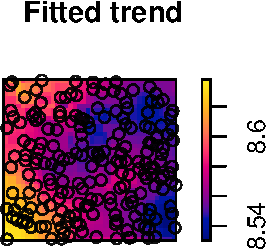
\includegraphics{Tutorial-spatstat_files/figure-beamer/unnamed-chunk-23-1} \end{center}
\end{frame}

\hypertarget{para-concluir}{%
\section{Para concluir}\label{para-concluir}}

\begin{frame}{Por hacer}
\protect\hypertarget{por-hacer}{}
\begin{itemize}
\item
  Verificar significancia de efectos
\item
  Verificar residuales (lo que el modelo no explicó)
\item
  Supuestos

  \begin{itemize}
  \tightlist
  \item
    Pertinencia del ``área de calibración''
  \item
    Supuesto de independencia rara vez se cumple
  \item
    Proponer modelos de interacción o gaussianos
  \end{itemize}
\end{itemize}
\end{frame}

\end{document}
